\documentclass[main.tex]{subfiles}

\begin{document}

\section{Filtro Adaptativo}
Al momento de elegir el algoritmo que se implementó para el filtro, 
se analizaron varias alternativas, entre ellas LMS, NLMS, VS-LMS y Sign LMS.
En primer lugar, los algoritmos Sign LMS, entre ellos, sign-error, sign-data
y sign-sign fueron descartados ya que el baud rate de la señal era de 250bps,
cabe recordar que esta variante de LMS es de utilidad para ecualizar canales de
comunicación digital de alta velocidad. En segundo lugar y  luego de analizar 
los resultados obtenidos y las conclusiones propuestas por Bismor \cite{bismor},
se decidió no implementar VS-LMS. En las palabras de los autores: 
"no hay algoritmo VS-LMS que sea tan versátil, fácil de implementar y adecuado 
para aplicaciones en tiempo real como el NLMS".\newline
Esta observación, si bien descarta la implementación de VS-LMS, 
plantea un último debate respecto a si corresponde utilizar LMS o NLMS. 
Se consideró entonces, analizar el parámetro de paso que se utilizaría para LMS. 
Se recuerda que el paso para que converja LMS está dado por
\begin{equation}
    0<\mu<\frac{2}{\lambda_\text{máx}}
\end{equation}
en donde $\lambda_\text{máx}$ es el autovalor más grande de $R$, la matriz de 
autocorrelación de $u(n)$. En la medida en que el  $\mu$ elegido se acerque 
al valor máximo, la velocidad de convergencia aumenta, pero así también el desajuste $\mathscr{M}$.
Por el contrario, al disminuir el paso, la convergencia se ralentiza, y disminuye $\mathscr{M}$. 
Se trata de una relación de compromiso entre la velocidad de convergencia y el desajuste.
Se realizaron 5000 simulaciones y se calculó el $\mu_\text{máx}$ para cada una de ellas.
Se muestra a continuación un histograma con la frecuencia de aparición del paso máximo, 
en función de este y los $\mu_\text{máx}$ en función del número de simulación.
\begin{figure}[H]
    \centering
    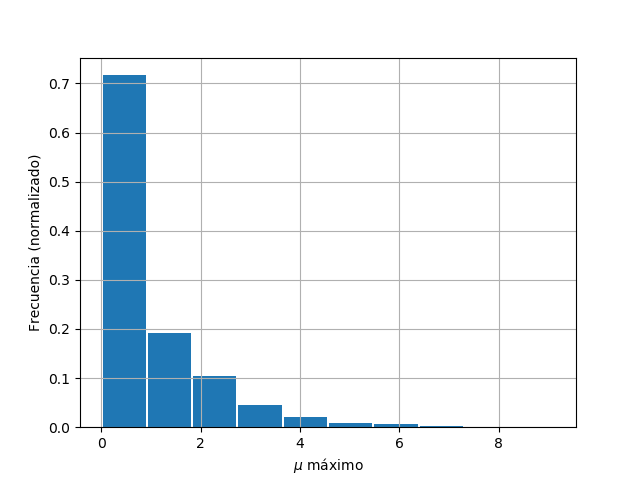
\includegraphics[scale=0.5]{imagenes/lms_mus_hist.png}
    \caption{Frecuencias de $\mu_\text{máx}$ en función del mismo.}
\end{figure}
\begin{figure}[H]
    \centering
    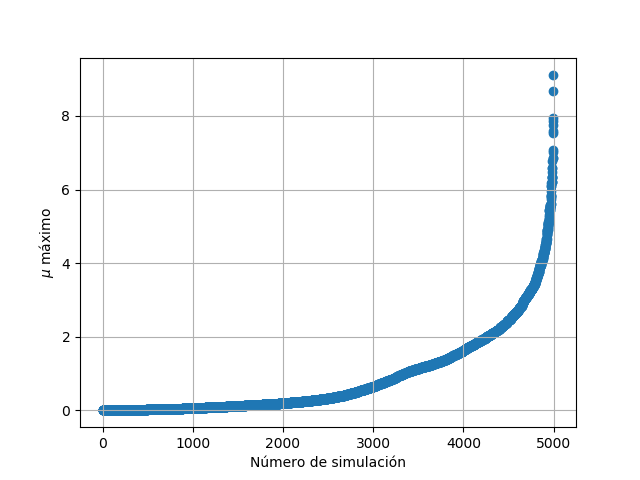
\includegraphics[scale=0.5]{imagenes/lms_mus_scatter.png}
    \caption{$\mu_\text{máx}$ en función del número de simulación.}
\end{figure}

El valor del parámetro de paso varía entre valores cercanos a 0 y mayores a 8, 
ya que las energías de la señal de entrada no están acotadas debido a las características 
del canal. Lo último presenta un problema al elegir el $\mu$ conveniente para la situación real,
puesto que si se elige un paso pequeño, tardará de manera considerable cuando el $\mu_\text{máx}$ sea alto;
y si se decide por un $\mu$ mayor, divergirá en los otros casos. \newline
Debido a lo expuesto anteriormente, se decidió no utilizar LMS, en pos de que no diverja el algoritmo. 
Esto se logró utilizando NLMS, pues lo que se introduce es un parámetro de paso variable, que depende
de la energía de la señal de entrada, por lo que la misma ya no es un problema.

\subsection*{NLMS}
\subsection*{Implementación}
\subsubsection*{Orden del filtro}
Como se mencionó en secciones anteriores, el canal es, si bien aleatorio, conocido, por 
lo que se pudo observar analizándolo que contaba con dos pares de polos conjugados, 4 polos.
Resulta entonces trivial la observación que con un filtro FIR de orden 4, los efectos 
de las singularidades se verían neutralizados. Se implementó entonces NLMS, y se realizó
una simulación de Montecarlo del bit error rate (BER) para órdenes de filtro entre 4, 5 y 6, en función del parámetro 
$\mu$.

\begin{figure}[H]
    \centering
    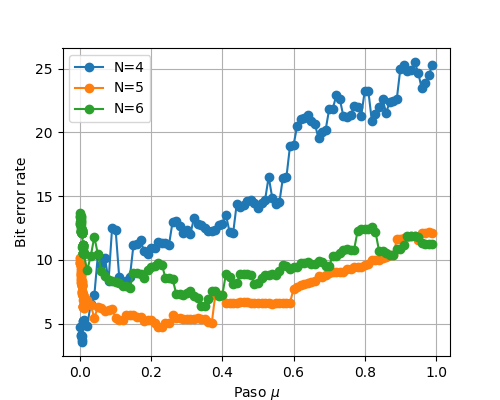
\includegraphics[scale=0.6]{imagenes/N_filter.png}
    \caption{Bit error rate en función de $\mu$ para orden 4, 5 y 6 del filtro.}
\end{figure}

Se observa que para valores de $\mu$ pequeños, el algoritmo mantiene un BER bajo 
para orden 4, desestabilizándose para pasos más grandes; no así ocurre con orden 5, 
que si bien tiene un mayor BER para valores bajos, tiene resultados más consistentes
para valores mayores de $\mu$. A su vez, este orden obtiene mejores resultados que un 
filtro de sexto orden. Con todo, el orden del filtro elegido fue 5.

\subsubsection*{Delay}
En lo que respecta al delay, bloque del esquema de inversión de sistemas, 
figura \ref{inversion-de-sistemas}, el retardo funciona como una compensación del delay real
del filtro y del canal. Además, es sólo utilizado para la secuencia de entrenamiento, para obtener la señal deseada.
En primer lugar se acotó el valor del delay entre 0-4 por el orden ideal del filtro, 
luego realizó un Montecarlo para estos valores de delay, donde nuevamente se
graficó el BER en función del parámetro de paso. Obteniendo una mejor tasa de error 
para el caso de delay unitario por lo que fue elegido.
\begin{figure}[H]
    \centering
    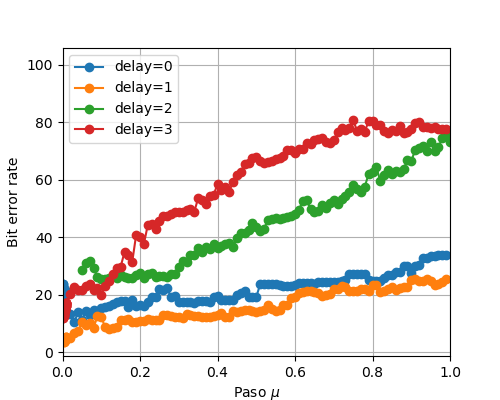
\includegraphics[scale=0.6]{imagenes/delay.png}
    \caption{Bit error rate en función de $\mu$ para delays entre 0-4.}
\end{figure}

\subsubsection*{Paso $\mu$}
De manera análoga, con base en ambos gráficos, se eligió un paso $\mu=0.005$; el valor
para el cual tanto para un  delay unitario, como para un filtro de quinto orden
el BER obtenido era menor al $5\%$.


\end{document}